\documentclass[a4paper, 11pt]{article}
\usepackage{amsmath}
\usepackage{amsfonts}
\usepackage{amssymb}
\usepackage{caratula}
\usepackage{listings}
\usepackage[utf8]{inputenc}
\usepackage[spanish, activeacute]{babel}
\usepackage[usenames,dvipsnames]{color}
\usepackage[width=15.5cm, left=3cm, top=2.5cm, height= 24.5cm]{geometry}
\usepackage{graphicx}
%\usepackage{subcaption}
\usepackage[all]{xy}
\usepackage{multicol}
\usepackage{subfig}
\usepackage{algorithm}
\usepackage{algorithmic}
\usepackage{cancel}
\usepackage{float}
\usepackage{xcolor}
\usepackage{color,hyperref}
\setcounter{secnumdepth}{3} %%agrego subsubsection

\lstset{breaklines=true, breakatwhitespace=true}
\lstset{numbers=left, numberstyle=\scriptsize}
\lstset{
     literate=%
         {á}{{\'a}}1
         {í}{{\'i}}1
         {é}{{\'e}}1
         {ý}{{\'y}}1
         {ú}{{\'u}}1
         {ó}{{\'o}}1
         {ě}{{\v{e}}}1
         {š}{{\v{s}}}1
         {č}{{\v{c}}}1
         {ř}{{\v{r}}}1
         {ž}{{\v{z}}}1
         {ď}{{\v{d}}}1
         {ť}{{\v{t}}}1
         {ñ}{{\~n}}1                
         {ů}{{\r{u}}}1
         {Á}{{\'A}}1
         {Í}{{\'I}}1
         {É}{{\'E}}1
         {Ý}{{\'Y}}1
         {Ú}{{\'U}}1
         {Ó}{{\'O}}1
         {Ě}{{\v{E}}}1
         {Š}{{\v{S}}}1
         {Č}{{\v{C}}}1
         {Ř}{{\v{R}}}1
         {Ž}{{\v{Z}}}1
         {Ď}{{\v{D}}}1
         {Ť}{{\v{T}}}1
         {Ň}{{\v{N}}}1                
         {Ů}{{\r{U}}}1    
}


%%%%%%%%%%%%%% ALGUNAS MACROS %%%%%%%%%%%%%%
% For \url{SOME_URL}, links SOME_URL to the url SOME_URL
\providecommand*\url[1]{\href{#1}{#1}}

\setlength{\parskip}{10pt plus 1pt minus 1pt}
\usepackage{tikz}
\def\checkmark{\tikz\fill[scale=0.4](0,.35) -- (.25,0) -- (1,.7) -- (.25,.15) -- cycle;}

% Same as above, but pretty-prints SOME_URL in teletype fixed-width font
\renewcommand*\url[1]{\href{#1}{\texttt{#1}}}

% Comando para poner el simbolo de Reales
\newcommand{\real}{\hbox{\bf R}}

\providecommand*\code[1]{\texttt{#1}}

%uso: \ponerGrafico{file}{caption}{scale}{label}
\newcommand{\ponerGrafico}[4]
{\begin{figure}[H]
	\centering
	\subfloat{\includegraphics[scale=#3]{#1}}
	\caption{#2} \label{fig:#4}
\end{figure}
}

\renewcommand{\algorithmiccomment}[1]{\hfill #1}

%%%%%%%%%%%%%%%%%%%%%%%%%%%%%%%%%%%%%%%%%%%%

\materia{Algoritmos y Estructuras de Datos III}

\titulo{TP1}
%\fecha{fecha de entrega}
%\grupo{Nro grupo}
\integrante{Sebastián Fernandez Ledesma}{392/06}{sfernandezledesma@gmail.com}
\integrante{Fernando Gasperi Jabalera}{56/09}{fgasperijabalera@gmail.com}
\integrante{Maximiliano Wortman}{892/10}{maxifwortman@gmail.com}
\integrante{Santiago Camacho}{110/09}{santicamacho90@gmail.com}


\include{templates}

\begin{document}
\pagestyle{myheadings}
\maketitle
%\markboth{Nombre materia}{Nombre TP}

\thispagestyle{empty}
\tableofcontents

%\setcounter{section}{-1}

\newpage
\section{Problema 1: Puentes sobre lava caliente}

\subsection{Presentaci\'on del problema}
%aca ponemos una interpretacion de lo que nos pide el enunciado y algunas aclaraciones de como vamos a encarar el problema.
Se quiere atravesar un puente con $n$ tablones dando saltos acotados por un valor de $x$ tablones. Se empieza afuera del puente y se pretende salir completamente de éste, es decir que como mínimo hay que saltar una vez (en el caso trivial de que $x > n$). La dificultad consiste en que ciertos tablones conocidos están rotos, y no pueden ser pisados. Lo que pide el problema es minimizar la cantidad de saltos para atravesar el puente, o aclarar que es imposible. Los puentes estarán definidos como $t_1$ $t_2$ $...$ $t_n$ donde $t_i = 0$ si el tablón está sano o $t_i = 1$ si está dañado. \\
Por ejemplo, podríamos tener el puente 0 1 0 0 con un salto máximo igual a 2. Como se arranca afuera, saltar al primer tablón se considera como un salto de 1 tablón. En este caso no podemos saltar los dos tablones permitidos porque el segundo tablón está roto (el puente, usando $X$ para marcar donde estamos parados, se vería así: X 1 0 0). El segundo salto sí podremos saltar los 2 tablones, quedando 0 1 X 0, y con el tercer salto saldremos del puente. \\
Una configuración más complicada podría ser el puente 0 0 1 0 0 0 1 1 0 0 para un salto máximo de 3 tablones, ya que ahora tenemos dos posibilidades: saltar al primer o al segundo tablón. Usaremos un algoritmo goloso para resolver el problema (saltar la mayor cantidad posible de tablones) y demostraremos que es correcto y que es la solución óptima para el problema.


\subsection{Resoluci\'on}
\subsubsection{Algoritmo}
%aca ponemos una descripcion de nuestro algorimtmo, presentamos la variables las estructuras y decimos que hacemos.
Dado este problema de optimización planteamos resolverlo con un algoritmo goloso, que consiste en seguir ``una heurística consistente para elegir la opción óptima en cada paso local con la esperanza de llegar a una solución general óptima'' [Cormen p.414 (Greedy Algorithms)].
El problema a optimizar es encontrar la mínima cantidad de saltos para cruzar el puente, y la decisi\'on golosa o la opcion \'optima en cada paso local es elegir el tabl\'on m\'as lejano que pueda alcanzar el participante de acuerdo al rango de salto que tenga. 

El algoritmo recibe un vector con los tablones del puente (puente$[i]$) y un entero que representa el máximo salto que puede dar el participante (\textit{maxSalto}).

Teniendo esa informaci\'on inicializamos la variable \textit{actual} y \textit{proximo} en $0$, que son enteros. La primera representa en que posici\'on del puente se ubica el participante y la segunda la posici\'on del salto m\'as lejano que puede alcanzar a un tablon.
Estas variables son actualizadas por un ciclo, que en el caso que haya soluci\'on corre hasta que la posici\'on \textit{actual} sea mayor a la cantidad de tablones, es decir que el participante haya cruzado el puente.

Dentro del ciclo, se calcula la variable \textit{proximo} con una funci\'on (\textit{calcularProximoTablon}) que recibe el \textit{puente} la posici\'on \textit{actual} y el \textit{maxSalto} y prueba desde el salto m\'as largo que puede dar hasta el m\'inimo cual es el pr\'oximo tablon \'optimo, si no existe, entonces devuelve una excepci\'on y hace que el algoritmo termine o en caso contrario el ciclo lo guarda en un vector de \textit{saltos}.
\textit{Actual} se actualiza a la posici\'on \textit{proximo} en cada iteraci\'on que significa que el participante avanza en cada vuelta del ciclo.

Una vez que termina el ciclo el algoritmo devuelve el arreglo de \textit{saltos}, que es vacio si no existe soluci\'on.

\subsubsection{Pseudoc\'odigo}
%aca va el pseudocodigo del problema.
\begin{algorithm}[H]
\begin{algorithmic}[1]
%\STATE input: vector$<$int$>$ puente, int maxSalto 
%\STATE output: vector$<$int$>$ saltos
\STATE int cantidadTablones $\gets |puente| - 2$ \textcolor{CadetBlue}{// El vector tiene dos tablones más: tanto el primero como el último se consideran fuera del puente}
\STATE int actual $\gets 0$
\STATE int proximo $\gets 0$
\WHILE {actual $\leq$ cantidadTablones}
    \STATE proximo $\gets$ calcularProximoTablon(puente, actual, maxSalto)
    \IF {proximo $==$ $-1$}
        \RETURN vector vacío
    \ENDIF
    \STATE introducirAlFinal(saltos, proximo)
    \IF {proximo $>$ cantidadTablones}
        \RETURN saltos
    \ENDIF
    \STATE actual $\gets$ proximo
\ENDWHILE
\caption{cruzarPuente(vector$<$int$>$ puente, int maxSalto ) $\rightarrow$ vector$<$int$>$ saltos}
\end{algorithmic}
\end{algorithm}

\begin{algorithm}[H]
\begin{algorithmic}[1]
\STATE int cantidadTablones $\gets |puente| - 2$
\WHILE {maxSalto $>$ 0}
    \IF {actual $+$ maxSalto $>$ cantidadDeTablones}
        \RETURN cantidadDeTablones $+$ 1
    \ENDIF
    \IF {puente$[$actual $+$ maxSalto$]$ $==$ 0}
        \RETURN actual $+$ maxSalto
    \ENDIF
    \STATE maxSalto $\gets$ maxSalto $-$ 1
\ENDWHILE
\RETURN $-1$
\caption{int calcularProximoTablon(vector$<$int$>$ puente, int actual, int maxSalto )}% $\rightarrow$ int proximo}
\end{algorithmic}
\end{algorithm}
\subsection{Demostraci\'on}
%aca va la demostracion formal del problema refiriendonos al pseudocodigo o redefiniendo variables (definir todas las cosas de las que vamos a hablar).
%MAXI

Vamos a tratar de probar que dado una secuencia de saltos, si para cada salto $s$, $s$ es un salto m\'aximo, y si la sumatoria de saltos es mayor a la cantidad de tablones del puente, entonces nuestra secuencia es solucion del problema.

Dada un Sec$<$Salto$>$ $se$.

$(\forall i:Nat, i < se.long)(esMax(s,i) \wedge \sum_{j=0}^{se.long-1}se_{j} = puente.long)\implies$ \\ $\not\exists (se':Sec<Salto>) /
se.long < se'.long \wedge \sum_{j=0}^{se'.long-1}se'_{j} \geq puente.long)$  

Dado s:Secuencia$<Salto>$, i:Nat esMax(s,i) devuelve true cuando no existe un salto mas largo desde la posicion $p$ donde estamos, donde posicion es la sumatoria de elementos hasta el elemento i.
 
%implementar esto.

Para probar esto, vamos a utilizar la definici\'on can\'onica de demostraci\'on de correctitud para algoritmos greedy, dada en clase por la c\'atedra. Un algoritmo goloso, puede plantearse como el siguiente esquema:
%comentar introduction to algorithim

\begin{algorithm}
\begin{algorithmic}
%\STATE input: S, F, P 
%\STATE output: S
\STATE $S^{opt}$ $=$ $\emptyset$
\WHILE {S $!=$ $\emptyset$}	
    \STATE X = $f(S)$
    \STATE S = $S - {X}$
    \IF {p($S^{opt}$,X)}
    \STATE $S^{opt} = S^{opt} \cup$ ${X}$   
    \ENDIF         
\ENDWHILE
\RETURN $S^{opt}$
\end{algorithmic}
\end{algorithm}

Luego para garantizar la correctitud del mismo hay que garantizar 4 puntos:

%comentar que esta sacada de la clase practica del dia xxxxxxx.
%esto deberia estar con indices, no con numeros cabeza

1) Definimos una noci\'on de lo que significa ser “sub-soluci\'on” de una soluci\'on.

2) Probar que $S^{opt}$ empieza siendo sub-soluci\'on de alguna soluci\'on \'optima.

3) Probar que si  $S^{opt}$ es sub-soluci\'on de alguna soluci\'on \'optima al iniciar 	una iteraci\'on del ciclo, entonces al terminar  esa iteraci\'on, $S^{opt}$ sigue siendo una subsoluci\'on de alguna soluci\'on \'optima.

4) Probar que cuando S $== \emptyset$, $S^{opt}$ es una soluci\'on \'optima.

Bueno para probar estos 4 puntos, primero vamos a definir F, S y P.


S es un conjunto de los saltos que uno puede dar representados por los pares (x,y) de tal que el representa un salto desde la posicion x hasta la posicion y con 0$<$ y-x$\leq$salto m\'ax.

F es una funci\'on que selecciona de S el par con mayor diferencia (y - x) y menor coordenada x.

P($S^{opt}$,X) devuelve TRUE cuando el tabl\'on donde cae X no esta roto y cuando el salto no se superpone con un salto anterior.
%Puente[$\sum_{i=0}^{S^{opt}.long}S^{opt}_{j}$ + X] $==$ 0 
%Donde Puente es el array de tablones, donde un tabl\'on esta sano si su valor es 0.

Vamos a definir ser sub-soluci\'on como ser el prefijo de una soluci\'on cuando ordenamos por orden de saltos.

Como la cantidad de saltos que puede darse en un puente es finita, va existir al menos un m\'aximo local y vamos a poder asignarle un cardinal. Entonces como existe al menos un conjunto de saltos de cardinal \'optimo, el conjunto $\emptyset$ empieza siendo sub-soluci\'on de ese conjunto.

Con esto queda comprobado 1) y 2).

Dado $S^{opt}$ sub-soluci\'on al principio del ciclo, queremos garantizar que $S^{opt}$ es sub-soluci\'on al finalizarlo.
Supongamos que $S^{opt}$ es sub-soluci\'on de $S^{*}$ al principio del ciclo.
Bueno si a $S^{opt}$ no le agrego nada, sigue siendo una subsolucio\'on.
Si el caso es en el que agrego X, quiero ver que eso sigue siendo alguna sub-soluci\'on para alg\'un $S'^{*}$. En particular queremos ver que $S'^{*}$ $\subset$ $S^{*}$. 
Si agregamos X, es el caso en donde P dio true, por lo tanto X cae en un tabl\'on que no esta roto y el salto no se superpone con uno anterior.
Adem\'as X era el m\'aximo de los saltos posibles y de menor coordenada x obtenido por F.
Bueno, si X $\in$ $S^{*}$, entonces podemos tomar $S'^{*}$ = $S^{*}$, asi que veamos el caso en que X $\notin$ $S^{*}$.

Ahora tomemos $S'^{*}$ = $S^{*}$ $\cup$ ${X}$
Este conjunto puede tener elementos que se superponen, si no los tiene entonces 
$S'^{*}$ es sub-soluci\'on.
Si los tiene, y ordenamos por orden de salto (primera coordenada) , $S'^{*}$ no puede superponerse con $S^{opt}$ ya que $S^{opt}$ era sub-soluci\'on de $S^{*}$.
Por lo tanto si existe un elemento que se superponga, se superponen con X.
Sea Y un elemento que se superpone con X.
Sean $Y_{1},Y_{2},X_{1},X_{2}$ las componentes de Y,X respectivamente.
$Y_{1}\geq X_{1}$ ya que sino X no tenia la primera componente m\'inima.

Si $Y_{1} = X_{1}$ entonces $X_{2} \geq Y_{2}$ ya que sino F hubiera agarrado primero a Y. 

Por lo tanto yo podria tomar $S'^{*}$ = $S^{*}$ $\cup$ ${X}$ - ${Y}$ y eso seguiria siendo sub-soluci\'on ya que el intervalo I = [$Y_{2},X_{2}$] estar\'ia cubierto con un solo salto por un soluci\'on que contenga a X, y necesitaria al menos 2 para un soluci\'on que contega a Y.

Si $Y_{1} > X_{1}$ entonces hay dos casos:

Si $Y_{2} \leq X_{2}$ entonces todo el intervalo cubierto por Y, estaria inclu\'ido en el intervalo cubierto por X, y en el intervalo I = [$X_{1},Y_{1}$], I $\neq \emptyset$ habr\'ia que cubrirlo con un salto por lo tanto $S^{*}$ no ser\'ia subsoluci\'on. Mismo para I' =  [$Y_{2},X_{2}$].

Si $Y_{2} > X_{2}$ entonces yo se que X,Y no pueden estar en la misma soluci\'on(se superponen). Pero se que Y pertenece a alguna soluci\'on. Veamos que existe un intervalo que cubre X, pero no Y que seria el intervalo I = [$X_{1}$,$Y_{1}$].
Bueno pero como X contiene a todo este intervalo, existe una solucion que contiene al salto $S_{Y}$ = ($X_{1}$,$Y_{1}$). Asi que dado un soluci\'on que contiene a Y, al menos contiene un salto m\'as en ese intervalo. Recordemos que puede haber saltos que extiendan el ultimo salto de $S^{opt}$, pero no nos interesan porque no ser\'ian compatibles con $S^{opt}$ ya que se superpondr\'ian.
 
Luego dado el intervalo I'=[$X_{2}$,$Y_{2}$], como X se superpone con Y, $X_{2}$ $>$ $Y_{1}$, por lo tanto existe y es posible un salto $S_{X}$ con componentes ($X_{2}$,$Y_{2}$).
Luego si analizamos las dos sub-soluciones contienen al mismo intervalo en dos saltos, por lo que si existe una soluci\'on para que contiene a Y, existe una soluci\'on que contenga a X. 

Con esto queda comprobado 3).

Finalmente, si S $== \emptyset$ entonces no hay mas saltos, por lo tanto nuestra $S^{opt}$ recorre e incluye a todo el puente.
Tenemos $S^{opt}$  que sabemos es una sub-soluci\'on de $S^{*}$. Y si $S^{opt}$ ya recorrio todo el puente, no hace falta agregarle ning\'un salto, por lo tanto $S^{opt} =S^{*}$.  

Con esto queda comprobado 4).
%MAXI
\\

------------------------------------------------------------------------\\
LIMPIADA DE CARA FER\\
------------------------------------------------------------------------\\
Definimos un salto $s$ como un natural mayor a 0 y menor o igual a la distancia 
máxima que puede recorrer el participante, de sólo un salto, medida en tablones

\begin{displaymath}
	s \in Saltos \Leftrightarrow (s \in \mathbb{N}_{> 0} \land s \leq dist_{max})
\end{displaymath}

Definimos un puente como una función $p: \mathbb{N}_{>0} \to \mathbb{N}$ 
\begin{displaymath}
	p(i) = \begin{cases} 
					1 &\mbox i \leq 0 \\ 
					0 &\mbox i > \#tablones \\
					0 &\mbox i > 0 \land i \leq \#tablones \land i \in Tablones \\
					1 &\mbox i > 0 \land i \leq \#tablones \land i \notin Tablones \\
				\end{cases} %\pmod{2}
\end{displaymath}

Para cada posición $i$ del puente definimos su salto máximo $s_{max}$ como 

\begin{displaymath}
	s_{max} = max \{n \in \mathbb{N}_{>0} \mid n \leq dist_{max} \land  \neg p(n)\}
\end{displaymath}

Nuestra implementacion recorre el puente dando saltos, garantizando que en cada salto, la distancia recorrida es m\'axima. Es decir, no existe otro salto tal que la distancia desde donde estamos parados es mayor a la del salto actual y el tabl\'on en el que caes no esta roto.\\
$Distancia$ es un Nat $>$ 0. \\
$Salto$ es Nat tal que $\forall s:Salto, s > 0 \wedge s \leq Distancia$
 
Vamos a tratar de probar que dado una secuencia de saltos, si para cada salto $s$, $s$ es un "salto maximo" y si la sumatoria de saltos es mayor a la cantidad de tablones del puente, entonces nuestra secuencia es solucion del problema.

Dada un Sec$<$Salto$>$ $se$.

$(\forall i:Nat, i < se.long)(esMax(se_{i}) \wedge \sum_{j=0}^{se.long-1}se_{j} = puente.long)\implies$ \\ $\not\exists (se':Sec<Salto>) /
se.long < se'.long \wedge \sum_{j=0}^{se'.long-1}se'_{j} \geq puente.long)$  //

Llamemos a sMax a la secuencia de saltos maximos obtenida.
Supongamos que existe secuencia s de saltos tal que la cantidad de elementos de s es menor a sMax y la sumatoria de saltos es igual o mayor a la cantidad de tablones.
Bueno en particular, existe al menos un salto $s_{i}$, tal que $s_{i}$, es mayor a $sMax_{i}$,  ya que si todos los $s_{i}$, son menores a su correspondiente $sMax_{i}$,
entonces la sumatoria de sMax es mayor que la sumatoria de s. (comprobar esto ad-hoc, probablemente sale por induccion).
Bueno, supongamos que agarro el primero de todos los $s_{i}$, que es mas grande que su correspondiente $sMax_{i}$.
Hasta ese momento las dos subsecuencias (desde el principio hasta el elemento i) pesan lo mismo, entonces $s_{i}$ esta parado en el mismo lugar y hace un salto mas grande que el salto maximo ($sMax_{i}$), lo cual es absurdo.
Por lo tanto queda comprobado que ese $s_{i}$, no puede existir y la solucion es m\'axima.

\subsection{An\'alisis de complejidad}
%aca decimos cuanto cuesta cada parte del algoritmo y damos un valor final de la complejidad del algoritmo, ej O(logn).
El algoritmo \textit{cruzarPuentes} se puede dividir en dos partes:
\begin{itemize}
\item Inicialización
\item Ciclo
\end{itemize}

En la Inicialización el algoritmo asigna 3 variables en $O(1)$, con lo cual su complejidad es $3*O(1) = O(1)$
El ciclo, como peor caso, itera hasta $n$ veces, donde $n$ es la \textit{cantidadDeTablones}. Adentro del ciclo se calcula la función \textit{calcularProximoTablon} para cada iteración. Esta nos dice el índice del próximo tablón óptimo para saltar, y a su vez es otro ciclo que se repite $k$ veces haciendo una cantidad acotada de operaciones $O(1)$, donde $k$ es la variable de entrada \textit{maxsalto} que es un valor acotado.
Luego el ciclo continua haciendo asignaciones y condicionales y devoluciones en $O(1)$.

Haciendo el calculo de complejidad obtenemos:

$O($\textit{cruzarPuentes}$) = 3*O(1) + n(O(k))$

Que es lo mismo que:

$O($\textit{cruzarPuentes}$) = O(n*k)$

%esto de decir que el algoritmo depende de k, yo no lo pondria porque sino nos van a decir que no es O(n) como pidieron ellos.

\label{an}
Podemos ver que la cota es todavia mejor.
Por cada paso que da, el algoritmo calcula hasta k tablones para saber cual es el pr\'oximo que no este roto m\'aximo, pero con la particularidad que calcula primero el mas lejano, por lo tanto dado un salto de longitud k':Nat, k'$\leq$ k, el pr\'oximo salto S, va a tener que ser mayor o igual a k - k', ya que sino S caeria en un tabl\'on roto.
Esto sucede porque k' esta acotado por los tablones que est\'an rotos.
Por ejemplo, suponiendo un k = 10. Dentro de un intervalo de tablones de 10 elementos, el tabl\'on 10, 9 y 8 est\'an rotos. Por lo tanto k' = 7. Entonces vemos que los tablones rotos por arriba son los que acotan a k', luego el pr\'oximo salto debe ser mayor a 3. Y si se itera mas de k - k' veces, el puente no tiene soluci\'on.
Esto lo que implica que dado cualquier k, el algoritmo siempre va a recorrer a lo sumo N elementos dentro del puente. El peor caso seria k=1.
Si a esto le agregamos la construcci\'on del array de entrada para el puente es de costo lineal en funci\'on de n, finalmente podemos concluir que todo el algoritmo es de orden $O(n)$.

\subsection{Test de complejidad}
%aca van los graficos y todos los testeos que hagamos para probar que en la practica el algoritmo cumple la complejidad que propusimos en el punto anterior

Para analizar y testear la complejidad del algoritmo implementado para la resoluci\'on del problema puentes colgantes realizamos los siguientes testeos:

\begin{itemize}
  \item Test de casos de tamaño fijo.
  \item Test de entrada al procesador.
  \item Test de analisis de peor caso.
\end{itemize}

\newpage



\subsubsection{Test de casos de tamaño fijo}


Para el test de complejidad utilizamos un algoritmo que genera un array de boolean aleatorios dado un k:Nat, tal que el largo del array es de tamaño k.

Luego generamos m:Nat arrays aleatorios de tamaño k. Dado un array $a$ se construye un puente $p$ el cual consta de los mismos elementos que el array aleatorio. 

$(\forall i:Nat, i < a.length)(a_{i} == p_{i})$

Luego se llama al algoritmo que obtiene la soluci\'on para ese puente.

Los tiempos medidos son a partir de que se llama al constructor del puente, y hasta despu\'es del llamado a nuestro algoritmo soluci\'on.

Para el test de casos de tamaño fijo, lo que usamos fue dadas las variables 

puenteMax:Nat, saltoMax:Nat, step:Nat, $cantidadDeIteraciones$:Nat. 

Vamos a iterar desde (i$=$step;i$<$puenteMax;i+=step), vamos a hacer $cantidadDeIteraciones$ instancias de puente y luego llamar al algoritmo de resoluci\'on con el procedimiento descrito arriba.

Luego dado un tiempo $T_{i}$ siendo este el promedio de todas las corridas de tamaño i, vamos a realizar un analisis de la complejidad obtenida.

Para el salto s:Nat que va a poder dar cada participante en cada instancia de puente tambien es un n\'umero aleatorio tal que

saltoMax:Nat, s $\leq$ saltoMax $\wedge$ saltoMax $<<$ i.

El siguiente gr\'afico muestra el crecimiento del $T_{i}$ en funci\'on de i, es decir el crecimiento del tiempo en funci\'on del crecimiento de elementos.
Los valores utilizados para la generaci\'on del grafico son:

\newpage

$cantidadDeIteraciones$ $=$ 100 step $=$ 50000 puenteMax $=$ 500000000 saltoMax = 10

\begin{figure}[ht]
	\begin{minipage}[t]{\linewidth}
		\centering
		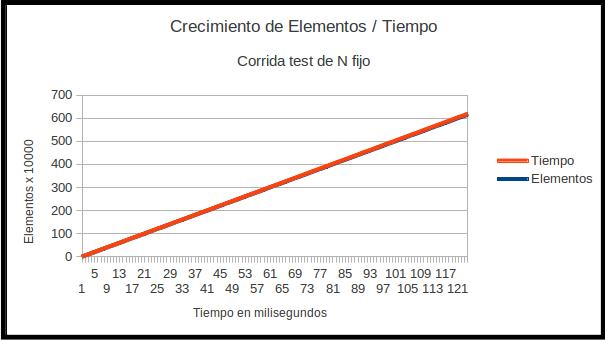
\includegraphics[width=\textwidth]{grafico_de_n_fijo.jpg}
	\end{minipage}	
\end{figure}

Como se puede apreciar la complejidad as\'intotica temporal en este caso, es lineal en el tamaño de la entrada.


\newpage
\subsubsection{Test de entrada al procesador}

El objetivo de este test era correr un test similar al test de tamaño fijo pero evitando los outlayers que pudiera generar el momento de entrada del problema al microprocesador. 

Para ello, lo que se implemento, fue correr una misma instancia de puente k veces y tomar ahora el promedio de esas k corridas similares, realizando el mismo proceso que en el test de tamaño fijo. Luego analizar en un gr\'afico la complejidad temporal de este test.

Los valores utilizados para la generaci\'on de este gr\'afico son:

$cantidadDeIteraciones$ $=$ 10 step $=$ 500000 puenteMax $=$ 500000000 saltoMax = 10 

k $=$ 10


\begin{figure}[ht]
	\begin{minipage}[t]{\linewidth}
		\centering
		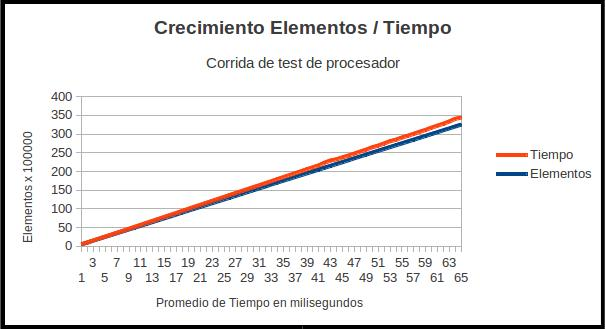
\includegraphics[width=\textwidth]{grafico_de_entrada_al_procesador.jpg}
	\end{minipage}	
\end{figure}

Como se puede apreciar la complejidad as\'intotica temporal en este caso, tambi\'en es lineal en el tamaño de la entrada.


\subsubsection{Test de peor-mejor caso}

Por lo analizado en demostraci\'on de correctitud, el peor caso va a ser cuando el salto m\'aximo s de un participante es s $=$ 1. Ya que este caso, de tener soluci\'on un puente p, se deber\'ia recorrer todos los tablones de p.

Luego la complejidad es exactamente N.

Los mejores casos ser\'ian lo que el salto m\'aximo s de un participante dado un puente p.

s $\geq$ p.largo

Ya que todo puente que el participante pueda saltar de un solo salto, tiene soluci\'on y nuestra implementaci\'on la haya en O(1).

\newpage

 
\subsection{Testing}
%aca ponermos todos nuestros casos bordes, como actua nuestro algoritmo en los casos particulares.

Para analizar y testear la correctitud del algoritmo implementado para la resoluci\'on del problema puentes colgantes realizamos los siguientes testeos:

\begin{itemize}
  \item Test de casos bordes.
  \item Test de archivos est\'aticos.
  \item Test de an\'alisis de input-output.
  \item Test de analisis generador de casos.
\end{itemize}

\subsubsection{Test de casos bordes}

Para los casos bordes de nuestro algoritmo elegimos correr una bater\'ia de test los cuales simulan casos at\'ipicos.
Los siguientes test fueron implementados:
Dado un puente p y participante con salto m\'aximo m.

\begin{itemize}
  \item TestConPuenteConTamanio0() $=$ Chequea soluci\'on para p.largo $=$ 0.
  \item 	TestConSaltoMaximo0() $=$ Chequea soluci\'on para s $=$ 0.
  \item TestConSaltoMaximoMayorAPuente() Chequea soluci\'on para s $\geq$ p.largo 
  \item testConPuenteNegativo() $=$ Chequea soluci\'on para p.largo $\leq$ 0
  \item testConSaltoNegativo() $=$ Chequea soluci\'on para s $\leq$ 0
\end{itemize}

\subsubsection{Test de archivos est\'aticos}

El objetivo de este test era probar la correctitud de nuestra implementaci\'on a partir de un archivo est\'atico de entrada y un archivo est\'atico de salida.
Estos archivos est\'atico de entrada y salida se los puede encontar en el directorio del programa bajo el nombre de ``puentes-estatico.txt" para la entrada y ``solucion-estatica" para la salida.

%hay que ponerle algunos casos mas a estos archivos%

\subsubsection{Test de an\'alisis de input-output}

El objetivo de este test era probar la correctitud del algoritmo de entrada de datos.
Se buscaba corroborar que la implementaci\'on correspondiera dada un archivo de entrada a la de un puente ya instanciado por el programa.
Para ello se genero un caso de test, el cual dado un puente creado aleatoriamente, crea un archivo de texto similar a los de entrada de la c\'atedra, con este puente. 

Luego se llamo con ese archivo a nuestra implementaci\'on de input, corroborando que la salida de este m\'etodo fuera similar a la de una llamada con el puente ya instanciado.

El test corre con k entradas de puentes generadas aleatoriamente.

\subsubsection{Test generador de casos}

El objetivo de este test es dado un puente p, generado aleatoriamente y dada la solucion s, corroborar que efectivamente si el algoritmo no devuelve soluci\'on entonces efectivamente no existe tal, y si la devuelve entonces s es soluci\'on del problema.

Para probar que no existe una soluci\'on para un puente p, vamos a aprovecharnos de una caracteristica de los puentes sin soluci\'on.

Para todo puente p sin soluci\'on dado un participante con salto m\'aximo m:Nat, y dados i,j:Nat, j-i $=$ m , existe un intervalo de tablones $[p_{i}$,$p_{j}]$ tal que para todo tabl\'on t dentro de ese intervalo, t est\'a roto.
La comprobaci\'on informal de este enunciado es que si no existiese ese intervalo, el participante siempre podria dar saltos al intervalo de tablones rotos que tiene adelante. Por lo tanto podr\'ia saltar por todo el puente.

Entonces dado un puente sin soluci\'on se chequea efectivamente que existe al menos un intervalo con estas caracter\'isticas.

Para corroborar que una s efectivamente es soluci\'on de p, vamos a iterar por los tablones de s y chequear en p, que estos no esten rotos.
Si bien esto no nos garantiza que s sea optima, nos garantiza que sea un camino posible de tablones.

Una mejora para estos test ser\'ia encontrar una caracter\'istica de s, tal que no asegure que es \'optima. Para ello, podr\'iamos generarnos por fuerza bruta todas las secuencias de saltos posibles y agarrar las que sean soluci\'on y garantizar que nuestra s es mejor o igual que todas las dem\'as (tiene menos elementos).

\subsection{Compilaci\'on y corrida}


La clase la cual debemos correr es Main, y debe tener un par\'ametro de entrada que sea el nombre del archivo del cual vamos a leer. \'Este archivo debe estar en el directorio del proyecto a en la carpeta ``TP1-EJ1", a la altura donde estan los dem\'as archivos de texto.
Para correr la clase Main, hay que posicionarse en el directorio bin del proyecto:

cd TP1-P1$/$bin

Luego desde este directorio con el comando java main/Main ..$/$$<$nombre de archivo$>$.

Ej: TP1-P1$/$bin java main$/$Main ../puente.txt

El output de esto deberia ser: 

3 2 4 6

no

 

\newpage
\section{Problema 2: Horizontes lejanos}

\subsection{Presentaci\'on del problema}
%aca ponemos una interpretacion de lo que nos pide el enunciado y algunas aclaraciones de como vamos a encarar el problema.
Dado un conjunto de rectángulos en un plano, todos apoyados sobre una linea recta horizontal, como en las siguientes figuras, se pide eliminar las líneas que colisionen con algún otro rectángulo, donde colisionar también es sólamente ``tocar'' otra línea.
\begin{figure}[ht]
	\begin{minipage}[t]{0.5\linewidth}
		\centering
		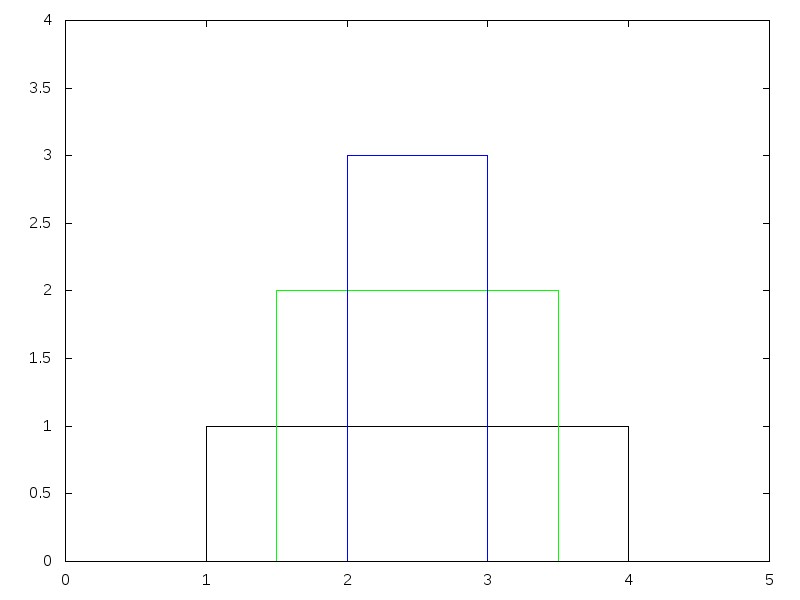
\includegraphics[width=\textwidth]{p1_ej1_pre.jpg}
		\caption{Con colisión total}
		\label{fig:p1_ej1_pre}
	\end{minipage}
	\begin{minipage}[t]{0.5\linewidth}
		\centering
		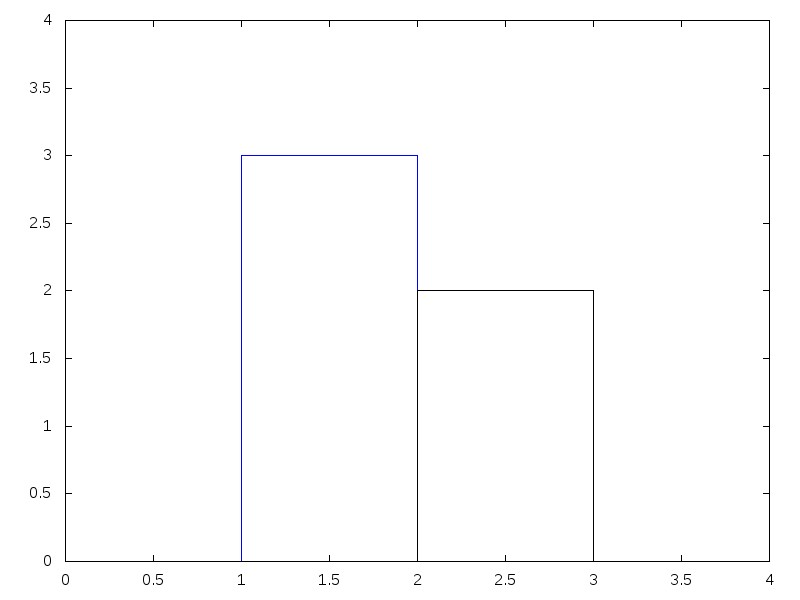
\includegraphics[width=\textwidth]{p1_ej2_pre.jpg}
		\caption{Sólo se tocan los bordes}
		\label{fig:p1_ej2_pre}
	\end{minipage}
\end{figure}

\noindent Así, tras ejecutar el algoritmo, el resultado para los ejemplos anteriores sería:

\begin{figure}[ht]
	\begin{minipage}[t]{0.5\linewidth}
		\centering
		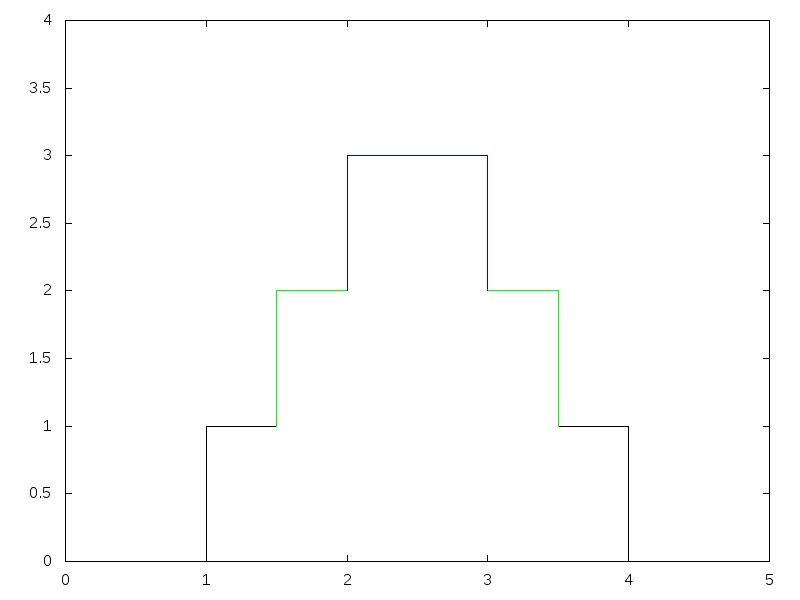
\includegraphics[width=\textwidth]{p1_ej1_post.jpg}
		\caption{Resultado con colisión total}
		\label{fig:p1_ej1_post}
	\end{minipage}
	\begin{minipage}[t]{0.5\linewidth}
		\centering
		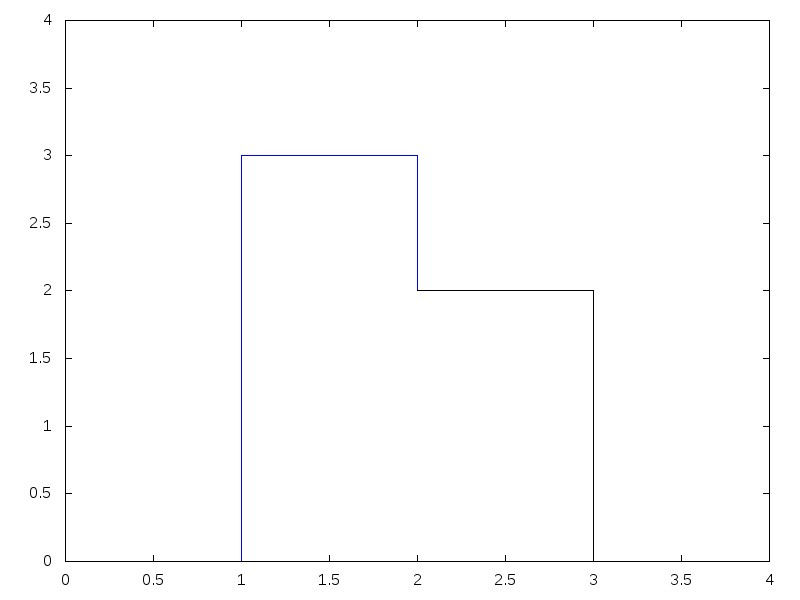
\includegraphics[width=\textwidth]{p1_ej2_post.jpg}
		\caption{Resultado cuando sólo se tocan los bordes}
		\label{fig:p1_ej2_post}
	\end{minipage}
\end{figure}

Como requerimiento adicional, el algoritmo para $n$ rectángulos debe tener una complejidad temporal estrictamente menor que $O(n^2)$.

\subsection{Resoluci\'on}
\subsubsection{Algoritmo}
Como introducción al pseudocódigo de nuestra implementación describiremos las ideas que lo respaldan para facilitar 
la asimilación del mismo. El algoritmo es muy simple pero tiene un par de puntos sutiles sobre los
que vale la pena hacer hincapié. A grandes rasgos se basa en los siguientes puntos:
\begin{enumerate}
	\item divide a los edificios en eventos de apertura y cierre
	\item ordena los eventos convenientemente
	\item itera el conjunto de eventos y va a agregando a su solución parcial los puntos en los que
	identifica cambios de altura (forma en la que definimos los puntos del contorno)
\end{enumerate} 
Cada edificio se representa con un evento de apertura y uno de cierre. Los dos eventos van a compartir la altura
original del edificio pero van a diferir en la coordenada $x$ que van a llevar: uno se quedará con la correspondiente
al inicio del edificio y el otro con la correspondiente a la finalización del mismo. 
El orden es más fácil pensarlo como una suerte de Radix Sort. Primero se ordena los eventos por su coordenada
$x$. Luego entre, entre los que comparten su coordenada $x$, se deja primero a los eventos de apertura y luego
a los de cierre. Finalmente, entre los que comparten coordenada $x$ y tipo, se ordena: en orden decreciente de altura
a los de tipo apertura y en orden creciente a los de tipo cierre. Vamos a mostrar la conveniencia de este orden
mostrando casos en los que traería problemas si estuvieran desordenados con respecto al criterio que recién describimos:
\begin{itemize}
	\item desordenados con respecto a $x$: tenemos dos edificios $e^1$ y $e^2$ superpuestos de forma tal que
	$e^1_p < e^2_p < e^1_f < e^2_f$ y $e^1_h > e^2_h$. Si iteramos primero $e^2$ vamos a suponer que en el comienzo
	del mismo hay un punto del contorno porque $e^1$ todavía no sabemos que estaba abierto.
	\item mismo $x$, desordenados respecto al tipo: suponemos que los eventos están todos correctamente ordenados
	con respecto a su coordenada $x$, sin embargo, dentro de los que comparten una misma coordenada $x$ a veces primero
	se colocó a los de cierre y luego a los de apertura. El problema que puede traer esto es que cuando yo veo
	un evento de cierre que era el que daba la altura máxima al contorno para obtener la nueva altura del contorno
	me fijo en los edificios que está abiertos. Si no cuento en ese momento con todos los que están abiertos
	en ese $x$ entonces puede que registre que el punto del contorno es diferente de lo que debería haber sido
	de saber que los que todavía no iteré de apertura estaban abiertos.
	\item eventos de apertura en orden creciente: supongamos que sólo tenemos 3 edificios, los 3 empiezan en
	la misma coordenada $x$ y los itero en orden creciente de altura. Cada vez que itero por uno de los eventos 
	de apertura me va a decir que la nueva altura es mayor a la que ya tengo del contorno por lo cual va a
	ingresar un nuevo punto al contorno, resultando en 3 puntos del contorno con el mismo $x$.
	\item eventos de cierre en orden decreciente: es muy similar al anterior, necesito haber cerrado los más
	bajos primero porque si no cuando cierro el más alto pienso que los que se van a cerrar en esa misma
	coordenada $x$ todavía están abiertos cuando en realidad no están abiertos en esa coordenada $x$, simplemente
	como los eventos se computan de a uno el orden es muy importante.
\end{itemize}
Además, queremos aclarar que para saber en todo momento qué edificios están abiertos mantenemos actualizada
una estructura con ésta información. La estructura no contiene los edificios que están abiertos, contiene
las alturas de los edificios que están abiertos. Con esta información basta ya que en todo momento
a nosotros nos interesa saber qué alturas tenemos disponibles para nuestro contorno, independientemente
del edificio al que pertenezcan. Cuando iteramos sobre un evento de apertura agregamos su altura a la 
estructura, cuando iteramos sobre un evento de cierre eliminamos un elemento con valor igual a la altura
del mismo.

\subsubsection{Pseudoc\'odigo}
%aca va el pseudocodigo del problema.
\begin{algorithm}[H]
\begin{algorithmic}
\STATE $eventos$ $\gets$ extraer\_eventos($edificios$)
\STATE $contorno_{parcial}$ $\gets$ $secuencia\_vacia$
\STATE $h_{actual}$ $\gets$ 0
\WHILE {$eventos$ $\neq$ $\emptyset$}
	\STATE $ev$ $\gets$ proximo\_evento($eventos$)
	\IF {abre($ev$)}
		\IF {$h_{actual}$ $<$ $ev_h$}
			\STATE $h_{actual}$ $\gets$ $ev_h$
			\STATE AgregarAtrás($<ev_x, ev_h>$, $contorno_{parcial}$)
		\ENDIF
	\ELSE
		\IF {$h_{actual}$ = $ev_h$ $\land$ maxAbierto($ev_x$) $<$ $h_{actual}$}
			\STATE $h_{actual}$ = maxAbierto($ev_x$)
			\STATE AgregarAtrás($<ev_x, h_{actual}>$, $contorno_{parcial}$)  
		\ENDIF
	\ENDIF
\ENDWHILE
\caption{horizontes\_lejanos}
\end{algorithmic}
\end{algorithm}

\begin{algorithm}[H]
\begin{algorithmic}
	\STATE $min_x$ = min( $\{ ev_x | ev \in eventos\}$ )
	\STATE $comparten\_min_x$ = $\{ ev \in eventos | ev_x = min_x \}$
	\IF {quedanEventosDeApertura($comparten\_min_x$)}
		\STATE $comparten\_min_x$ = filtrarLosDeCierre($comparten\_min_x$)
		\RETURN mayorAltura($comparten\_min_x$)
	\ELSE
		\RETURN menorAltura($comparten\_min_x$)
	\ENDIF
\caption{proximo\_evento}
\end{algorithmic}
\end{algorithm}

\subsection{Demostraci\'on}
\paragraph{Edificio}
Definiremos un edificio $e$ como una tupla $<e_{principio}$, $e_{final}$, $e_{altura}>$, la escribiremos de la siguiente forma por ser más compacta $<e_p$, $e_f$, $e_h>$, que cumple la siguiente propiedad:
\begin{displaymath}
	e_p, e_f, e_h \in \mathbb{N} \land e_p > 0 \land e_p < e_f \land e_h > 0
\end{displaymath}
La misma representa a un edificio $e$ que empieza en $e_p$, tiene una altura de $e_h$ y termina en $e_f$. 
Representados bidimensionalmente sobre un eje cartesiano los valores $e_p$ y $e_f$ se corresponden con
sus coordenadas sobre el eje de las abscisas $X$.

\paragraph{Evento}
Definiremos un evento como una tupla $<ev_x$, $ev_h$, $ev_t>$ que cumple la siguiente propiedad:
\begin{displaymath}
	ev_x, ev_h, ev_t \in \mathbb{N} \land ev_t \in \{ 1, 0\}
\end{displaymath}
$ev_x$ representa el valor de la coordenada $x$ del evento, $ev_h$ la altura del evento y $ev_t$ el tipo de 
evento, 1 para un evento que representa el comienzo de un edificio y 0 para los eventos que representan el fin de un edificio.
Dado un edificio $e = <e_p$, $e_f$, $e_h>$  diremos que dos eventos lo representan $ev_{abrir} = <e_p$, $e_h$, $1>$ y $ev_{cerrar} = <e_f$, $e_h$, $0>$.
Es decir, que cada edificio lo representamos con dos eventos, uno que marca el comienzo y otro que marca el fin del mismo. 
Dado un conjunto $E$ de edificios decimos que el conjunto $Ev$ de eventos que lo representa es aquel que contiene dos eventos
por cada edificio de $E$ derivados de la forma antes mostrada.

\paragraph{Contorno}
Dado un conjunto de edificios $E$ definiremos una función $h$ que toma un $x \in \mathbb{N}$ y un conjunto de edificios:
\begin{displaymath}
	h: (x,E) \to \mathbb{N} 
\end{displaymath}
$h$ nos devuelve la altura del edificio más alto que cubre ese valor de $x$ 
\begin{displaymath}
	h(x, E) = \begin{cases} 
						0 & \nexists e \in E | (x \geq e_p \land x < e_f) \\
						max\{ e_h | e \in E  \land e_p \leq x \land x < e_f \} & \exists e \in E | (x \geq e_p \land x < e_f)
				\end{cases} %\pmod{2}
\end{displaymath}
contando con $h$ ya podemos definir correctamente nuestro conjunto de puntos que conforman el contorno del
conjunto de edificios $E$:
\begin{displaymath}
	C = \{ p \in \mathbb{N}^2 | h(p_x - 1, E) \neq h(p_x, E) \land (\exists ev \in Ev | ev_x = p_x \land ev_h = p_y) \}
\end{displaymath}
Es decir, los puntos que pertenezcan al conjunto $contorno$ registrarán los cambios de altura. Cada punto
del contorno puede interpretarse como: a partir de este $p_x^i$ y hasta el $p_x^{i+1}$ el edificio con mayor
altura en todo el rango tiene altura igual a $p_y^i$ (asumiendo que los $p^i$ del contorno están ordenados
de forma creciente por su coordenada $x$). Los cambios de altura pueden producirse
porque un edificio empiece o porque un edificio haya concluido. 
Dado un conjunto de edificios $E$ existe un único conjunto $C$ que representa su contorno. 
Vale la pena aclarar que por como está planteado el problema la función $h$ nos dice que si tenemos un conjunto $E$
de edificios que sólo contiene un edificio $e = <e_p, e_f, e_h>$ entonces $h(e_p, E) = e_h$ pero $h(e_f, E) = 0$.
La altura de los edificio representa de esta forma un intervalo cerrado a izquierda pero abierto a derecha
respecto a la información que el contorno registra.

\textbf{Correctitud}
\par
A continuación se presenta el pseudocódigo de nuestra implementación sobre el cual plantearemos la
demostración de correctitud:

De ahora en más vamos a referirnos como $contorno$ a la secuencia que contiene a todos los elementos de
el conjunto de contorno $C$ ordenados por su coordenada $p_x^i$. Además, vamos a referirnos a que un
edificio $e$ contiene o abarca a un valor $x$ cuando $x \in [e_p, e_f)$.

Vamos a demostrar algunos lemas que nos servirán para realizar la demostración.

\paragraph{Lema 1}
Todos los puntos pertenecientes a $C$ satisfacen:
\begin{enumerate}
	\item $(\forall p \in C) \exists ev \in Eventos \text{ / } p_x = ev_x$
\end{enumerate}
La propiedad se desprende de la misma definición del conjunto $contorno$. Como $h(p_x, Edificios) \neq h(p_x - 1, Edificios)$ 
necesariamente ese cambio en la función de altura tiene que haberse producido porque un edificio 
$e = <e_p$, $p_x$, $h(p_x-1, Edificios)>$ concluyó, en el caso de que $h(p_x, Edificios) < h(p_x - 1, Edificios)$, o porque un
edificio $e = <p_x$, $e_f$, $h(p_x, Edificios)>$ comenzó, en el caso de que $h(p_x, Edificios) > h(p_x - 1, Edificios)$, ya que 
la altura por defecto para cualquier valor de $x$ que no esté contenido por un edificio del conjunto de edificios es 0. En los dos
casos tenemos un edificio que empieza o termina en $p_x$. Como el conjunto $Eventos$ contiene precisamente un evento por cada comienzo
y fin de un edificio, en particular contiene a los que satisfacen en cada caso la propiedad expresada.

\paragraph{Lema 2}
Sea S la secuencia de eventos tal que:
\begin{displaymath}
	ev \in S \Leftrightarrow ev \in Eventos
\end{displaymath}
de forma tal que el orden en el que se encuentran es el impuesto por agregarlos en el orden en el que la función 
proximo\_evento($Eventos$) los devuelve. Se cumple que:
\begin{displaymath}
	(\forall ev^1, ev^2 \in Eventos \text{ / } ev^1_x = ev^2_x) ev^1_h * ev^1_t > ev^2_h * ev^2_t \Rightarrow posicion(ev^1, S) < posicion(ev^2, S)
\end{displaymath}
Los casos que podemos tener son los siguientes:
\begin{enumerate}
	\item $\text{abre}(ev^1) \land \neg\text{abre}(ev^2)$  en este caso vemos que necesariamente $ev^1$ va a ser devuelto
	primero por proximo\_evento() porque siempre si los eventos comparten la coordenada $x$ prioriza los de apertura
	con la función filtrarLosDeCierre(Eventos).
	\item $\text{abre}(ev^1) \land \text{abre}(ev^2)$  podemos ver en el algoritmo de proximo\_evento() que cuando luego
	de filtrar por $min_x$ y quedarse con los de apertura en caso de que existan, estamos en el caso de que existen,
	$ev_1$ y $ev_2$ cumplen, devuelve primero el de mayor altura. Con lo cual la posición del de mayor altura
	necesariamente es menor.
\end{enumerate}
$\square$

\paragraph{Lema 3}
Sea $contorno$ la secuencia de puntos del contorno $C$ ordenados por su coordenada $x$. La secuencia tiene 
$n+1$ puntos $p^0,...,p^n$:
\begin{displaymath}
	(\forall x \in \mathbb{N} \text{ / } x < p_x^0 \lor x \geq p_x^n) h(x, E) = 0
\end{displaymath}
y además:
\begin{displaymath}
	(\forall x \in \mathbb{N} \text{ / } x \geq p_x^0 \land x < p_x^n) h(x, E) = p_y^{maxXmenor}
\end{displaymath}
con $p_y^{maxXmenor}$ igual al $p_y$ del $p$ que tiene el máximo $p_x$  de todos los $p$ que cumplen $p_x \leq x$.

La primer propiedad predica que antes del primer edificio y después del último, asumiendo un orden por coordenada $x$,
la función $h$ siempre vale 0. Estose desprende directamente de su definición, si todavía no empieza ningún edificio o
si ya terminaron todos es imposible que la altura valga algo mayor a 0 porque por defecto vale 0.
La segunda propiedad nos dice que entre dos puntos $p^1$, $p^2$ consecutivos del contorno la función $h$ necesariamente tiene
que devolvernos $p_y^1$. Si no fuera así entonces existiría un $x$ entre $p_x^1$ y $p_x^2$ en el cual $h(x, Edificios)$ nos devuelve
distinto de $p_y^1$. Como $p_y^1 = h(p^1_x, Edificios)$, por definición de contorno debería existir un punto $p$ del mismo
tal que $p_x = x$. Pero $x$ se encuentra entre $p_x^1$ y $p_x^2$ que son puntos consecutivos del contorno por lo cual no
puede existir ningún cambio de altura entre ellos ya que si existiera debería haber un punto del contorno allí y eso es
absurdo porque presumimos que eran consecutivos.
$\square$
 
Nuestro algoritmo consiste en un ciclo que itera sobre todos los elementos de $Eventos$. Vamos a demostrar
que el ciclo cumple el siguiente invariante:
\begin{displaymath}
	esPrefijo(contorno_parcial, contorno) 
\end{displaymath}

\textbf{Antes de entrar al ciclo}
\par
Antes de entrar al ciclo $contorno_{parcial} = secuencia\_vacia$. La secuencia vacía es prefijo de todas las secuencias, por lo tanto
el invariante se cumple antes de entrar al ciclo por primera vez.
\par
\textbf{El ciclo preserva el invariante}
\par
Si el ciclo no agrega puntos a $contorno_parcial$ entonces necesariamente sigue siendo prefijo de $contorno$ por lo cual
el invariante se preserva. Necesitamos demostrar que lo preserva cuando agrega elementos al mismo. Llamamos $p^i$ al último 
elemento de la secuencia $contorno_{parcial}$ y $h_{actual}$ a $p^i_y$. Existen dos casos en los que agrega elementos a 
$contorno_parcial$, estos son cuando se cumplen alguna de estas dos proposiciones:
\begin{description}
	\item[Caso 1] $\text{abre}(ev) \land h_{actual} < ev_h$
	\item[Caso 2] $\neg\text{abre}(ev) \land ev_h = h_{actual} \land maxAbierto(ev_x) < h_{actual}$
\end{description}
$contorno_{parcial}$ es prefijo de $contorno$. Para que $contorno_{parcial}$ continue siendo prefijo el elemento
que agregue tiene que ser necesariamente $p^{i+1}$ en la secuencia $contorno$. $p^{i+1}_x$ es el mínimo $x$ tal que $x > p^i_x$
 y $h(x, Edificios) \neq p^i_y$. Por \textbf{Lema 1} sabemos que necesariamente existe un $ev$ tal que $ev_x = p^{i+1}_x$.
\par
Si $p^{i+1}_x > p^{i}_x$ entonces vale abre($ev$). Por \textbf{Lema 2} sabemos que nuestro algoritmo
iterará primero sobre el $ev^i$ con $ev^i_x = p^{i+1}_x \land \text{abre}(ev^i)$ de mayor altura. Entonces, necesariamente itera
primero sobre el que cumple que $ev_x = p^{i+1}_x \land h_{actual} < ev_h$. Como entra en el Caso 1 sabemos que lo va a agregar y además
sabemos que como proximo\_evento() devuelve primero los que menor coordenada $x$ tengan será el con mínimo $ev_x$ que cumple el Caso 1.
Entonces concluimos que si $p^{i+1}_x > p^{i}_x$ entonces nuestro algoritmo lo va a agregar a contorno parcial y va a ser el
primero que agregue. Por lo tanto, $contorno_{parcial}$ sigue siendo prefijo de $contorno$.
\par
El otro caso es cuando vale $p^{i+1}_x < p^{i}_x$. Ésto implica que $\neg\text{abre}(ev)$, tomando $ev$ con el que se 
corresponde con $p^{i+1}$. $ev_h = h_{actual}$ se desprende de que si fuera mayor caemos en un absurdo porque asumimos que 
$p^{i+1}_x < p^{i}_x$ y si fuera menor entonces no cambiaría la altura, lo cual lo excluiría de la definición de los 
puntos pertenecientes a $C$. Por último, es necesario que $maxAbierto(ev_x) < h_{actual}$ porque si no se cumpliera
esto no existiría tal cambio de altura, por lo cual el punto no pertenecería la contorno. Por lo tanto, el próximo punto
del contorno cae en nuestro Caso 2 y también es agregado al $contorno_{parcial}$ para que preserve la propiedad
de ser prefijo de $contorno$.
\par
Finalmente, necesitamos demostrar que la satisfacción del invariante y la negación de la guarda del ciclo implican que 
$contorno_{parcial} = contorno$. Veamos que:
\begin{enumerate}
	\item Comparten el último elemento: el último elemento de $contorno$ cumple que $p_y = 0 \land p_x = e_f^max$ con $e_f^max$
	el maximo valor de finalizacion de entre todos los edificios. Antes de $e_f^max$ $h \geq e_h^max$ y para todo $x$ mayor o igual
	a $e_x^max$ valdrá 0. Por lo tanto, es el último punto donde cambia la altura, será el último punto de mi contorno. Ese punto
	además tiene un evento correspondiente que es el último que recorre proximo\_evento() y cumple el Caso 2 por lo
	cual también será agregado.
	\item El orden que guardan sus elementos es total: esto ya lo demostramos, es simplemente que $p^i_x < p^{+1}i_x$ para 
	todos los i entre 0 y las longitud de $contorno$. 
\end{enumerate}
Estas dos propiedades y el hecho de que sea prefijo una de otra nos implica directamente que las secuencias son iguales. Por
lo tanto, al concluir el ciclo, efectivamente $contorno_{parcial} = contorno$.

\subsection{An\'alisis de complejidad}
Para calcular la complejidad del algoritmo que implementamos primero debemos
explicar cómo resolvimos en la implementación el cáculo de maxAbierto($x$) con
una estructuras de datos conveniente que nos permite realizar todas las
operaciones necesarias sin superar la cota de complejidad requerida.
Contamos con un Multiconjunto, que llamaremos $abiertos$, que nos provee la
siguiente interfaz:
\begin{itemize}
	\item inserción: $O(log n)$
	\item borrado: $O(log n)$
	\item obtención del máximo: $O(log n)$
\end{itemize}
utilizaremos esta estructura de forma tal que calcular la función maxAbierto($x$)
sea equivalente a obtener el máximo de este multiconjunto. Para ello debemos
mantenerlo actualizado, esto implica que en cada iteración si el evento es de tipo
apertura lo agregamos a $abiertos$ (costo O($log n$)). 

La complejidad de este algoritmo puede calcularse como:
\begin{displaymath}
	O(extraer_eventos) + \#eventos * O(proximo_evento) + 
\end{displaymath}


\subsection{Test de complejidad}
%aca van los graficos y todos los testeos que hagamos para probar que en la practica el algoritmo cumple la complejidad que propusimos en el punto anterior

\subsection{Testing}
%aca ponermos todos nuestros casos bordes, como actua nuestro algoritmo en los casos particulares.

































\newpage
\section{Problema 3: Biohazard}

\subsection{Presentaci\'on del problema}
%aca ponemos una interpretacion de lo que nos pide el enunciado y algunas aclaraciones de como vamos a encarar el problema.

\subsection{Resoluci\'on}
\subsubsection{Algoritmo}
%aca ponemos una descripcion de nuestro algorimtmo, presentamos la variables las estructuras y decimos que hacemos.

\subsubsection{Pseudoc\'odigo}
%aca va el pseudocodigo del problema.

\subsection{Demostraci\'on} %OPCIONAL
%aca va la demostracion formal del problema refiriendonos al pseudocodigo o redefiniendo variables (definir todas las cosas de las que vamos a hablar).

\subsection{An\'alisis de complejidad}
%aca decimos cuanto cuesta cada parte del algoritmo y damos un valor final de la complejidad del algoritmo, ej O(logn).

\subsection{Test de complejidad}
%aca van los graficos y todos los testeos que hagamos para probar que en la practica el algoritmo cumple la complejidad que propusimos en el punto anterior

\subsection{Testing}
%aca ponermos todos nuestros casos bordes, como actua nuestro algoritmo en los casos particulares.


\newpage
\section{Apéndice: Códigos fuente}

\subsection{Problema 1: Puentes sobre lava caliente}

Código del algoritmo que resuelve el problema:
\lstset{language=C++,
                keywordstyle=\color{blue},
                stringstyle=\color{red},
                commentstyle=\color{magenta},
                morecomment=[l][\color{magenta}]{\#}
}
\begin{lstlisting}[frame=single]
vector<int> cruzarPuente(int puente[], int cantidadDeTablones, int largoSalto)
{
    int actual = 0, proximo = 0;
    vector<int> saltos;
    while (actual <= cantidadDeTablones) {
        proximo = calcularProximoTablon(puente, cantidadDeTablones, actual, largoSalto);

        if (proximo == IMPOSIBLE) return vector<int>();

        saltos.push_back(proximo);

        if (proximo > cantidadDeTablones) return saltos;

        actual = proximo;
    }
}

// Dado un puente y un tablón devuelve cuál es el salto más largo que se puede realizar desde ese tablón. Si no puede realizarse ningún salto devuelve IMPOSIBLE(-1).
int calcularProximoTablon(int puente[], int cantidadDeTablones, int actual, int largoSalto)
{
    while (largoSalto > 0) {
       if (actual + largoSalto > cantidadDeTablones) 
           return cantidadDeTablones+1;
       
       if (puente[actual+largoSalto] == 0)
           return actual+largoSalto;
           
       largoSalto--;
    }

    return IMPOSIBLE;
}
\end{lstlisting}

Por una cuesti\'on de tiempos, la implementaci\ testeada de este ejercicio esta en el leguaje Java. El algoritmo es similar a su implementaci\'on en c++.


Código de la implementaci\'on (en Java):
\lstset{language=Java,
                keywordstyle=\color{blue},
                stringstyle=\color{red},
                commentstyle=\color{magenta},
                morecomment=[l][\color{magenta}]{\#}
}
\begin{lstlisting}[frame=single]
int saltos = 0;
StringBuilder builder = new StringBuilder();
		if (saltoMax > 0) {
			int pos = 0;
			while (pos < puente.largo() + 1) {
				int i = saltoMax;
				boolean salte = false;
				while (i > 0 && !salte) {
					if (puente.estaRoto(i + pos)) {
						i--;
					} else {
						pos += i;
						builder.append(" " + pos);
						saltos++;
						salte = true;
						i = saltoMax;
					}
				}
				//fallo algun intervalo
				if (!salte) {
					return "no";
				}
			}
		}
		if (saltos != 0) {
			//existe sol		
			return saltos + builder.toString();
		}
		//fallo en el primer interavlo
		return "no";
\end{lstlisting}

Código de los tests de complejidad (en Java):
\lstset{language=Java,
                keywordstyle=\color{blue},
                stringstyle=\color{red},
                commentstyle=\color{magenta},
                morecomment=[l][\color{magenta}]{\#}
}
\begin{lstlisting}[frame=single]
// Este test lo vamos a utilizar para medir el tiempo que tarde en resolverse una entrada en el procesador. Para ello vamos a tratar de mediar una entrada resuelta k veces. El test va a ser similiar al de tamaño fijo pero corriendo cada instancia k veces.
public class TestDeEntradaAlProcesador {

    private static int PUENTEMAX = 500000000;

    private static Random random = new Random(new Date().getTime());

    private static int SALTOMAX = 10;

    private static int CANTIDADDECORRIDAS = 10;

    private static int CANTIDADDEIERACIONES = 10;

    public static void main(String[] args) {
        testEntradaAlProcesador();
    }

    public static void testEntradaAlProcesador() {
        for (int i = 500000; i < PUENTEMAX; i += 500000) {
            float prom = 0;
            for (int j = 0; j < CANTIDADDEIERACIONES; j++) {
                float promSubj = 0;
                int saltoMax = random.nextInt(SALTOMAX);
                boolean[] b = new boolean[i];
                for (int k = 0; k < b.length; k++) {
                    b[k] = random.nextBoolean();
                }
                for (int k = 0; k < CANTIDADDECORRIDAS; k++) {
                    Long ats = new Date().getTime();
                    Puente puente = new Puente(b);
                    Saltarin.saltar(puente, saltoMax);
                    Long dps = new Date().getTime();
                    promSubj += dps - ats;
                }
                prom += promSubj / (CANTIDADDECORRIDAS);

            }
            System.out.println(i / 100000 + "," + prom / CANTIDADDEIERACIONES);
        }
    }

}

public class TestDeTamanioFijo {

    private static int PUENTEMAX = 500000000;

    private static Random random = new Random(new Date().getTime());

    private static int SALTOMAX = 10;

    private static int CANTIDADDEIERACIONES = 100;

    // Este metodo lo utilizamos para medir tiempos, notamos que a partir de los 500000000 elementos la entrada comienza a tener un diferencia de tiempo (tF-tI) significante El primer valor es el N, el segundo una constante k la cual hace que se resuelven k puentes de tamaño N. El algoritmo de me devuelve el promedio de solucion de esos puentes. Luego hay una tercer constante m que es el tamanio del saltoMax, la implementacion genera un saltoMax aleatorio, pero que no puede ser mayor a m. Vamos a generar casos que tengan N >> saltoMax, ya que en esos casos se ve mas clara la complejidad.
    public static void main(String[] args) {
        testDeComplejidad();
    }

    public static void testDeComplejidad() {
        for (int i = 1; i < PUENTEMAX; i += 50000) {
            float prom = 0;
            for (int j = 0; j < CANTIDADDEIERACIONES; j++) {
                int saltoMax = random.nextInt(SALTOMAX);
                boolean[] b = new boolean[i];
                for (int k = 0; k < b.length; k++) {
                    b[k] = random.nextBoolean();
                }
                Long ats = new Date().getTime();
                Puente puente = new Puente(b);
                Saltarin.saltar(puente, saltoMax);
                Long dps = new Date().getTime();
                // Esto lo hacemos para evitar outlayers
                if (j > 10) {
                    prom += dps - ats;
                }
            }
            System.out.println(i / 10000 + "," + prom
                    / (CANTIDADDEIERACIONES - 10));
        }
    }
}
\end{lstlisting}

\subsection{Problema 2: Horizontes lejanos}

Código fuente del algoritmo que resuelve el problema:
\lstset{language=C++,
                keywordstyle=\color{blue},
                stringstyle=\color{red},
                commentstyle=\color{magenta},
                morecomment=[l][\color{magenta}]{\#}
}
\begin{lstlisting}[frame=single]
struct Edificio {
    int left;
    int right;
    int h;
};

enum tipos_de_eventos {EMPIEZA, TERMINA};
struct Evento {
   Evento() : edificio(0) {};
   Evento(tipos_de_eventos t, int x, int h, int edificio) : tipo(t), x(x), h(h), edificio(edificio) {};

   bool empieza() const { return tipo == EMPIEZA; };

   int edificio;
   tipos_de_eventos tipo;
   int x;
   int h;
};

struct Punto {
    Punto(int x, int y) : x(x), y(y) {};
    int x;
    int y;
};

int main(int argc, const char *argv[])
{
    int cantidadDeEdificios;
    while(true) {
        cin >> cantidadDeEdificios;
        if (cantidadDeEdificios == 0) return 0;

        vector<Edificio> edificios(cantidadDeEdificios);
        for (int i = 0; i < cantidadDeEdificios; i++) {
            edificios[i] = Edificio();
            cin >> edificios[i].left >> edificios[i].h >> edificios[i].right;

            assert(edificios[i].left >= 0);
            assert(edificios[i].h >= 0);
            assert(edificios[i].right >= 0);
            assert(edificios[i].left < edificios[i].right);
        }

        // cada edificio va a tener un evento de empezar y uno de terminar
        vector<Evento> eventos = generarEventos(edificios);
        // los eventos son ordenados por su coordenada x de forma ascendente
        // desempata por el tipo de evento, EMPIEZA gana
        sort(eventos.begin(), eventos.end(), &comparar_eventos_por_x);

        vector<Punto> contorno = calcularContorno(eventos);

        for (int i = 0; i < contorno.size(); i++) {
            cout << contorno[i].x << " " << contorno[i].y;
            if (i < (contorno.size()-1)) cout << " ";
        }
        cout << endl;
    }

    return 0;
}

vector<Punto> calcularContorno(const vector<Evento> &eventos)
{
    // alturas de edificios abiertos
    multiset<int> abiertos;
    multiset<int>::iterator itAbiertos;
    Evento eventoActual;
    int alturaContornoActual = 0;
    vector<Punto> contorno;

    for (int i = 0; i < eventos.size(); i++) {
        eventoActual = eventos[i];
        if (eventoActual.empieza()) {
            abiertos.insert(eventoActual.h);
            if (eventoActual.h > alturaContornoActual) {
                contorno.push_back(Punto(eventoActual.x, eventoActual.h));
                alturaContornoActual = eventoActual.h;
            }
        } else {
            // lo busco primero porque sólo quiero eliminar una aparición
            // y puede que haya más de un edificio abierto con la misma
            // altura
            itAbiertos = abiertos.find(eventoActual.h); 
            abiertos.erase(itAbiertos);
            if (eventoActual.h == alturaContornoActual) {
                int tempAltura = alturaContornoActual;
                alturaContornoActual = (abiertos.empty() ? 0 : *abiertos.rbegin());
                if (tempAltura != alturaContornoActual)
                    contorno.push_back(Punto(eventoActual.x, alturaContornoActual));
            }
        }
    }
    
    return contorno; 
} 

vector<Evento> generarEventos(const vector<Edificio> &edificios)
{
    int cantidadDeEdificios = edificios.size();
    vector<Evento> eventos(cantidadDeEdificios*2);
    for (int i = 0; i < cantidadDeEdificios; i++) {
        eventos[i*2] = Evento (EMPIEZA, edificios[i].left, edificios[i].h, i);
        eventos[i*2+1] = Evento (TERMINA, edificios[i].right, edificios[i].h, i);
    }
    
    return eventos;
}

bool comparar_eventos_por_x(const Evento &a, const Evento &b)
{
    if (a.x == b.x) {
        if (a.empieza() != b.empieza()) // distinto tipo => gana el de apertura
          return a.empieza();

        if (a.empieza()) { // son los dos de apertura
          return a.h > b.h;
        } else {           // son los dos de cierre
          return a.h < b.h;
        }
    }
    
    return a.x < b.x;
}
\end{lstlisting}

Código fuente del generador de instancias:
\begin{lstlisting}[frame=single]
int main(int argc, const char *argv[])
{
    srand (time(NULL));
    int i;
    for(i=1;i<=1000; i++)
    {
        for (int j = 0; j < 10; j++)
        {
            cout << i <<"\n";
            for (int k = 0; k < i; k++)
            {
                int y = rand() % (1000) + 2;
                int x = rand() % (y-1);
                int h = rand() % (1000);
                cout << x << " " << h << " " << y << "\n";
            }
            cout << "\n";
        }
    }
    cout << "0"; 
    return 0;
}
\end{lstlisting}

Código fuente del test (sólo se modifica \textbf{main}):
\begin{lstlisting}[frame=single]
int main(int argc, const char *argv[])
{
    int cantidadDeEdificios;
    int contador = 1;
    int sumaTiempos = 0;
    int tiempoParcial = 0;
    while(true) {
        cin >> cantidadDeEdificios;
        if (cantidadDeEdificios == 0) return 0;

        vector<Edificio> edificios(cantidadDeEdificios);
        for (int i = 0; i < cantidadDeEdificios; i++) {
            edificios[i] = Edificio();
            cin >> edificios[i].left >> edificios[i].h >> edificios[i].right;

            assert(edificios[i].left >= 0);
            assert(edificios[i].h >= 0);
            assert(edificios[i].right >= 0);
            assert(edificios[i].left < edificios[i].right);
        }
        for(int j = 0; j < 10; j++){
            auto start_time = chrono::high_resolution_clock::now();//TIEMPO
            // cada edificio va a tener un evento de empezar y uno de terminar
            vector<Evento> eventos = generarEventos(edificios);
            // los eventos son ordenados por su coordenada x de forma ascendente
            // desempata por el tipo de evento, EMPIEZA gana
            sort(eventos.begin(), eventos.end(), &comparar_eventos_por_x);

            vector<Punto> contorno = calcularContorno(eventos);
            auto end_time = chrono::high_resolution_clock::now();//TIEMPO
            tiempoParcial = tiempoParcial + chrono::duration_cast<chrono::nanoseconds>(end_time - start_time).count();//TIEMPO
        }
        
        tiempoParcial = tiempoParcial / 10; //divido la corrida de la misma instancia
        int sumaTiempos = sumaTiempos + tiempoParcial;
        if(contador == 10){
            sumaTiempos = sumaTiempos / 10;
            sumaTiempos = sumaTiempos / log(cantidadDeEdificios);
            cout << cantidadDeEdificios << " " << sumaTiempos / 10;
            cout << endl;
            contador=1;
            tiempoParcial = 0;
            sumaTiempos = 0;
        }
        contador++;

    }

    return 0;
}
\end{lstlisting}

\subsection{Problema 3: Biohazard}

Código fuente del algoritmo que resuelve el problema (con la poda de ``agregar camión''):
\lstset{language=C++,
                keywordstyle=\color{blue},
                stringstyle=\color{red},
                commentstyle=\color{magenta},
                morecomment=[l][\color{magenta}]{\#}
}
\begin{lstlisting}[frame=single]
struct Camion {
    Camion() : productos(set<int>()), peligrosidad(0) {};
    Camion(int producto) : peligrosidad(0) {
        productos = set<int>();
        productos.insert(producto);
    };

    set<int> productos;
    int peligrosidad;
};

int peligrosidades[1024][1024];

int main(int argc, const char *argv[])
{
    int n, umbralDePeligrosidad;
    int i = 1;
    while(true) {
        cin >> n;
        if (n == 0) return 0;
        cout << "Instancia " << i << endl;
        i++;
        cin >> umbralDePeligrosidad;

        for (int i = 0; i < n; i++) {
            for (int j = 0; j < n; j++) {
               if (i == j) peligrosidades[i][i] = 0;
               if (i < j) cin >> peligrosidades[i][j];  
               if (i > j) peligrosidades[i][j] = peligrosidades[j][i];
            }
        }

        vector<Camion> camiones;
        camiones.push_back(Camion(0));
        vector<Camion> solucion;
        for (int i = 0; i < n; i++) {
           solucion.push_back(Camion(i)); 
        }
        bt(1, camiones, solucion, umbralDePeligrosidad, n);
        
        int elementosCamiones[n];
        set<int>::iterator it;
        for(int i = 0; i < solucion.size(); i++) {
            for (it = solucion[i].productos.begin(); it != solucion[i].productos.end(); it++) {
                elementosCamiones[*it] = i;
            }
        }

        cout << solucion.size() << " ";
        for (int i = 0; i < n; i++) {
            cout << elementosCamiones[i];
            if (i < (n-1)) cout << " ";
        }
        cout << endl;
        
    }
    return 0;
}

void bt(int producto, vector<Camion> &camiones, vector<Camion> &mejorTemp,
    int umbral, int n)
{
    if (producto == n && camiones.size() < mejorTemp.size()) {
        mejorTemp = camiones;
        return;
    }
    if (producto == n) return;
    for (int j = 0; j < camiones.size(); j++) {
        if (agregarNoSuperaUmbral(producto, camiones[j], umbral)) {
            int peligrosidadPrevia = agregarProducto(producto, camiones[j]);
            bt(producto+1, camiones, mejorTemp, umbral, n);
            sacarProducto(producto, camiones[j], peligrosidadPrevia);
        }
    }
    if (camiones.size() < (mejorTemp.size()-1)) {
        camiones.push_back(Camion(producto));
        bt(producto+1, camiones, mejorTemp, umbral, n);
        camiones.pop_back();
    }

    return;
}

bool agregarNoSuperaUmbral(int producto, const Camion &camion, int umbral)
{
    int acumPeligrosidad = camion.peligrosidad;
    set<int>::iterator it;
    for (it = camion.productos.begin(); it != camion.productos.end(); it++) {
        acumPeligrosidad += peligrosidades[producto][*it];
        if (acumPeligrosidad > umbral) return false;
    }
    
    return true;
}

void sacarProducto(int producto, Camion &camion, int peligrosidadPrevia)
{
    camion.productos.erase(producto);
    camion.peligrosidad = peligrosidadPrevia;
}

int agregarProducto(int producto, Camion &camion)
{
    int peligrosidadPrevia = camion.peligrosidad;
    set<int>::iterator it;
    for (it = camion.productos.begin(); it != camion.productos.end(); it++) {
        camion.peligrosidad += peligrosidades[producto][*it];
    }
    camion.productos.insert(producto);
    
    return peligrosidadPrevia;
}
\end{lstlisting}

Código fuente del generador de instancias aleatorias:
\begin{lstlisting}[frame=single]
// Este programa va a crear una cantidad X de instancias aleatorias de N productos, para N = {1,...,algunValor} y las va a devolver por SALIDA ESTANDAR (consola). El umbral va a ser fijo. Vale que para toda peligrosidad, 0 <= peligrosidad <= UMBRAL + 1.
// Hay que usar ./randomGen > textFile para guardar a disco.
// g++ -O3 randomGen.cpp -o randomGen

#include <iostream>
#include <unistd.h>
#include <cstdlib>
#include <cstdlib>

using namespace std;

const int CANT_INSTANCIAS = 5;
const int LIM_PRODUCTOS = 15;
const int UMBRAL = 100;

int main(int argc, const char* argv[]) {
    srand(time(NULL) + getpid()); // Seedeo
    for (int totalProductos = 2; totalProductos <= LIM_PRODUCTOS; totalProductos++) {
        for (int instancia = 1; instancia <= CANT_INSTANCIAS; instancia++) {
            cout << totalProductos << " " << UMBRAL << endl;
            for (int producto = 1; producto <= totalProductos - 1; producto++) {
                for (int peligrosidad = 1; peligrosidad <= totalProductos - producto; peligrosidad++) {
                    cout << rand() % (UMBRAL + 2) << " "; // Esto genera un entero random entre 0 y UMBRAL + 1.
                }
                cout << endl;
            }
        }
    }
    cout << "0" << endl;
}
\end{lstlisting}

Código fuente del test de complejidad (sólo se modifican la función \textbf{bt} y \textbf{main}):
\begin{lstlisting}[frame=single]
// Dado un archivo de entrada con X instancias para cada N cantidad de productos (N <= 100), devuelvo por SALIDA ESTANDAR, en cada linea, lo siguiente:
// N <espacio> promedio{ los minimo{ tiempos en ejecutar la instancia i-ésima para N productos } de todas las instancias de N productos}
// Es decir, cada instancia se ejecutará una cierta cantidad de veces y se tomará el mínimo para mejorar la precisión, y luego se promediaran estos valores para las instancias de cada cantidad de productos.
// g++ -std=c++0x p3-test.cpp -o p3-test
#include <climits>
#include <iostream>
#include <vector>
#include <set>
#include <chrono>

using namespace std;

const int MAX_CANTIDAD_PRODUCTOS = 100;
const int FOR_MINIMO = 2;
const bool PODA_AGREGAR_CAMION = true;
const bool PODA_RESTO_PRODUCTOS = true;

int peligrosidades[MAX_CANTIDAD_PRODUCTOS][MAX_CANTIDAD_PRODUCTOS];

int main(int argc, const char *argv[])
{   
    int sumaTiemposPorCantProductos[MAX_CANTIDAD_PRODUCTOS + 1] = { }; // Pongo cada tiempo en su casilla correspondiente, ie tiempo para i productos en suma[i]
    int cantidadInstanciasPorCantProductos[MAX_CANTIDAD_PRODUCTOS + 1] = { }; // Idem para la cantidad de instancias, esto lo uso para promediar
    int n, umbralDePeligrosidad;
    while(true) {
        cin >> n;
        if (n == 0) break;
        cin >> umbralDePeligrosidad;

        for (int i = 0; i < n; i++) {
            for (int j = 0; j < n; j++) {
               if (i == j) peligrosidades[i][i] = 0;
               if (i < j) cin >> peligrosidades[i][j];  
               if (i > j) peligrosidades[i][j] = peligrosidades[j][i];
            }
        }
        
        chrono::microseconds minTiempo(INT_MAX);
        for (int i = 0; i < FOR_MINIMO; i++) {
            // Acá considero que arranca el algoritmo
            auto start_time = chrono::high_resolution_clock::now();
            vector<Camion> camiones;
            camiones.push_back(Camion(0));
            vector<Camion> solucion;
            for (int i = 0; i < n; i++) {
               solucion.push_back(Camion(i)); 
            }
            bt(1, camiones, solucion, umbralDePeligrosidad, n);
            // Acá terminó
            auto end_time = chrono::high_resolution_clock::now();
            chrono::microseconds temp = chrono::duration_cast<chrono::microseconds>(end_time - start_time);
            if (temp < minTiempo)
                minTiempo = temp;
        }
        sumaTiemposPorCantProductos[n] += minTiempo.count();
        cantidadInstanciasPorCantProductos[n]++;
    }
    
    for (int i = 2; i <= MAX_CANTIDAD_PRODUCTOS; i++) {
        int instancias = cantidadInstanciasPorCantProductos[i];
        if (instancias == 0) {
            continue;
        } else {
            cout << i << " " << sumaTiemposPorCantProductos[i] / instancias << endl;
        }
    }
    return 0;
}

void bt(int producto, vector<Camion> &camiones, vector<Camion> &mejorTemp,
    int umbral, int n)
{
    if (producto == n && camiones.size() < mejorTemp.size()) {
        mejorTemp = camiones;
        return;
    }
    if (producto == n) return;
    for (int j = 0; j < camiones.size(); j++) {
        if (agregarNoSuperaUmbral(producto, camiones[j], umbral)) {
            int peligrosidadPrevia = agregarProducto(producto, camiones[j]);
            if (PODA_RESTO_PRODUCTOS) { // PODA DE RESTO DE LOS PRODUCTOS //
                if (camiones.size() == mejorTemp.size() - 1) {
                    //cout << "PODA PRODUCTOS" << endl;
                    for (int i = producto + 1; i < n; i++) {
                        bool entraEnAlguno = false;
                        for (int c = 0; c < camiones.size(); c++) {
                            if (agregarNoSuperaUmbral(i, camiones[c], umbral)) {
                                entraEnAlguno = true;
                                break;
                            }
                        }
                        if (!entraEnAlguno) {
                            sacarProducto(producto, camiones[j], peligrosidadPrevia);
                            continue;
                        }
                    }
                }
            }
            bt(producto + 1, camiones, mejorTemp, umbral, n);
            sacarProducto(producto, camiones[j], peligrosidadPrevia);
        }
    }
    if (PODA_AGREGAR_CAMION) { // PODA DE AGREGAR CAMION //
        if (camiones.size() == mejorTemp.size() - 1) {
            //cout << "PODA CAMIONES" << endl;
            return;
        }
    }
    camiones.push_back(Camion(producto));
    bt(producto+1, camiones, mejorTemp, umbral, n);
    camiones.pop_back();

    return;
}
\end{lstlisting}


\newpage
% Bibliografía
\addcontentsline{toc}{section}{Referencias}
\bibliography{tp3.bib}{}
\bibliographystyle{acm}

\end{document}
